\documentclass[10pt]{article}
\usepackage[margin=0.6in]{geometry}
\usepackage{amsmath}
\usepackage{booktabs}
\usepackage{xcolor}
\usepackage{graphicx}
\usepackage{hyperref}
\usepackage{titlesec}
\usepackage{enumitem}
\usepackage{tcolorbox}

\definecolor{navy}{RGB}{31,42,89}
\definecolor{teal}{RGB}{20,110,120}
\definecolor{findbg}{RGB}{240,246,248}

\titleformat{\section}{\large\bfseries\color{navy}}{\thesection}{0.6em}{}
\titlespacing*{\section}{0pt}{10pt}{4pt}
\pagenumbering{gobble}

\newtcolorbox{finding}[1][]{colback=findbg,colframe=teal,boxrule=0.6pt,left=6pt,right=6pt,top=3pt,bottom=3pt,#1}

\begin{document}

\begin{center}
{\small\textcolor{teal}{\bfseries REVIEW 1 --- ONE-PAGE SUMMARY}}\\[2pt]
{\Large\bfseries\color{navy} Temperature-Compensated PLL Frequency Synthesizer in sky130}\\[2pt]
{\small Aaryan Dogra (23BEC1032) \quad Yugeshwaran (23BEC1404) \quad Viju Sanjai (23BEC1306) \quad Guide: Dr. B. Bindu}
\end{center}
\vspace{2pt}

\section{What changed and why}
No local Cadence license $\Rightarrow$ rebuilt the flow open-source: hand-written SPICE, ngspice, SkyWater sky130 PDK, fully headless (no GUI). Added a full schematic-to-GDS scope (original brief was schematic-only) and reframed the contribution around a literature-checked research question rather than reproducing a known circuit.

\section{The hypothesis}
Temperature compensation is a \emph{cancellation} problem: a correction network subtracts two large drift terms to leave a small residual, which amplifies simulator/model disagreement by roughly the compensation ratio $C$. \textbf{H1:} $\varepsilon_{\text{res}} \approx C \cdot \varepsilon_{\text{raw}}$, implying a trust ceiling on how deep a correction an open-source flow can be relied on to design. Tested via cross-validation against Cadence/Spectre (Review 3).

\section{Circuit built (all transistor-level except the charge pump)}
\begin{center}
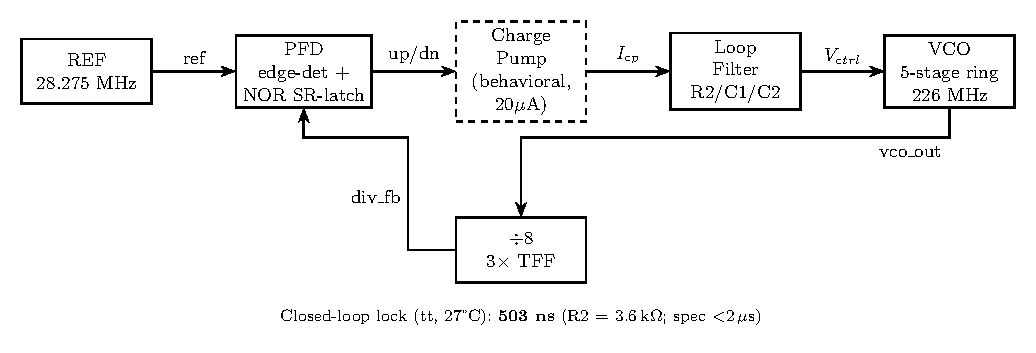
\includegraphics[width=0.98\textwidth]{diagrams/pll_block_diagram.pdf}
\end{center}

\section{Key results}
\begin{center}
\small
\begin{tabular}{lll}
\toprule
\textbf{Quantity} & \textbf{Measured} & \textbf{Target / Reference} \\
\midrule
Closed-loop lock time & \textbf{577 ns} & $<2\,\mu$s spec; 450 ns analytical prediction \\
Settled VCO / divider frequency & 227.96 / 28.515 MHz & 226.2 / 28.275 MHz target \\
$K_{VCO}$ (fit @ 0.9V) & $\approx$670 MHz/V & curve is nonlinear, not a bare secant \\
Uncompensated tempco, ff / tt / ss & 332 / 681 / 1070 ppm/$^\circ$C & $>3\times$ spread across corners \\
Divider ratio (measured) & 8.004 & target 8.000 \\
\bottomrule
\end{tabular}
\end{center}

\section{What we proved wrong (our own inherited spec, not the reference papers)}
\begin{itemize}[leftmargin=1.3em, itemsep=1pt]
  \item \textbf{``$\pm0.15$\,ppm stability''} is not physically meaningful for a reference-locked PLL ($f_{out}=N f_{ref}$ exactly in lock) $\to$ restated as \textbf{$<\pm0.3\%$ residual VCO drift}, grounded against Souliotis et al.\ 2022's fabricated $-1.5\%/+0.4\%$.
  \item \textbf{$V_{ctrl}$ floor of 0.27\,V} is unreachable --- this ring-VCO is device-threshold-limited, measured floor $\approx$0.6--0.65\,V $\to$ spec revised to \textbf{0.63\,V}.
  \item A single scalar compensation ratio $C$ doesn't hold given the $>3\times$ corner spread $\to$ \textbf{$C$ locked as per-corner}.
\end{itemize}

\section{What we took from the reference papers, and what we added}
\begin{itemize}[leftmargin=1.3em, itemsep=1pt]
  \item \textbf{Souliotis et al.\ 2022}: the PTAT/CTAT-compensated ring-VCO topology class (not claiming novelty here).
  \item \textbf{Freitas et al.\ 2025 (TWEPP)}: closest prior open-vs-commercial comparison, but theirs is \emph{open-loop and qualitative only} $\to$ we close the loop and (Review 3) make it quantitative.
  \item \textbf{Thiriloganathan et al.\ 2026 (SMACD)}: confirms open-source tools have no PSS/Pnoise $\to$ we plan the same transient/jitter workaround, honestly labelled as an estimate.
\end{itemize}

\begin{finding}
\textbf{Bottom line:} the loop locks, in budget, with the analytical model agreeing to the right order of magnitude, and every specification gap found was caught with real simulation data, not assumed. Full detail, all raw numbers, and two documented root-cause debugging stories: \texttt{RESULTS.md} and \texttt{review1\_report.pdf} in the project repository.
\end{finding}

\end{document}
